\documentclass[a4paper]{article}
\usepackage{a4wide}
\usepackage{fancyhdr}
\usepackage{scrextend}
\usepackage{coordsys,logsys,color}
\usepackage[bookmarksopen,bookmarksdepth=5]{hyperref}
\usepackage{url}
\usepackage{texdraw}
\usepackage{graphicx}
\usepackage{wrapfig}
\usepackage{listings}
\usepackage{diagbox}
\usepackage{enumitem}
\usepackage{amssymb}
\usepackage{amsmath}
\usepackage{float}
\usepackage{tikz}
\usepackage{longtable}
\usepackage{booktabs}
\usepackage{ltxtable}
\usepackage{cleveref}
\usepackage[backend=biber]{biblatex}
\usepackage{minted}

\NeedsTeXFormat{LaTeX2e}
\definecolor{darkblue}{rgb}{0,0,.6}
\hypersetup{colorlinks=true, breaklinks=true, linkcolor=black, menucolor=darkblue, urlcolor=darkblue, citecolor=darkblue}

\pagestyle{fancy}
\rhead{}

\setlength{\headheight}{23pt}
\bibliography{resources.bib}

\begin{document}
\begin{titlepage}
\thispagestyle{plain}
   \begin{center}
       \vspace*{1cm}
        \Huge
       \textbf{Local Field Potential Analysis Software} \vspace*{3em} \\
       \normalsize
               \textbf{Abstract: \\}
        TODOs:
        \begin{itemize}
        \item Abstract
         \item Figures/Wireframes
         \item References/Bibliography
         \item Refinement of SW design: Code structure, what functions from where, interfaces used, $\dots$
        \end{itemize}
        
        
        \vfill
       
       
       Fabian Klopfer \vspace{1em}\\
       Experimental Neurophysiology of Channelopathies \& \\ Molecular and Translational Neurosurgical Epileptology Research Groups \vspace{1em} \\
       Department of Neurology and Epileptology \vspace{1em} \\
       Hertie Institute for Clinical Brain Research \vspace{1cm} \\
       
\includegraphics[keepaspectratio, height=0.1\textheight]{img/logo.png}
        \vspace*{1cm}
        
   \end{center}
\end{titlepage}

\tableofcontents
\section{Software Requirements \& Design}
	\subsection{Purpose \& Scope}
		The purpose of this piece of software is to enable researchers in the Lerche lab to analyze local field potentials recorded with multi electrode arrays. 
		Foremost it shall focus on the analysis of the data recorded with the Multicannel systems MEA2100-HS256 headstage and the Multichannel systems 256MEA200/30iR-ITO chip of a wild type and a SCN1A mutant A1783V. 
		Further models may be recorded and analyzed. 
		The system shall incorporate methods that assist in the inspection and quantification of differences in neural activity between A1783V mutants and wild type mice during baseline and seizure/seizure-like conditions. 
		Concretely it shall assist in answering the questions how far, how fast, with what magnitude and with which subcomponents a seizure-like firing activity spreads upon the presentation of a stimulus with NMDA, 4AP and Mg deprived solution.
	
    \subsection{Definitions, Acronyms, Abbreviations}
	\begin{longtable}{>{\raggedright \arraybackslash}p{0.35\textwidth}
	>{\raggedright \arraybackslash}p{0.15\textwidth}>{\raggedright \arraybackslash}p{0.5\textwidth}} \toprule
	term & shortform & meaning \\ \midrule
	Power spectral density &  PSD & Distribution of average power of a signal in the frequency domain. Power present in the signal as a function of frequency \\
	Multi-electrode array & MEA & A multi-electrode array is a grid of tightly spaced microscopic electrodes embedded in the bottom of each well. MEAs are devices that contain multiple microelectrodes through which neural signals are obtained or delivered, essentially serving as neural interfaces that connect neurons to electronic circuitry.  \\
    Peristimulus time histogram & PSTH & A PSTH is a histogram wich usually specifies how often a population neuron fires in a certain amount of time and at a certain point in time. \\ \bottomrule
	\end{longtable}
	
	\subsection{Product Perspective \& User Characteristics}
		The system shall run on all platforms and shall be easy to use for researchers without extensive background in computer science. 
		A basic level of data science, that is statistics, signal processing and machine learning techniques is required to a level where the user knows what methods intuitively do, but not to a level of algorithmic or implementation understanding. 
		Users are too expected to have basic skills in the Python programming language.

	\subsection{Functional Requirements}
	 The system shall enable
		\begin{enumerate}
		 \item the visual exploration of data,
		 \item the selection of channels,
		 
		 \item the extraction of 
		 \begin{itemize}
		  \item localised power spectrum densities,
		  \item as well as time series of PSDs,
		 \end{itemize}

		 \item the splitting of spectra into periodic and aperiodic components,
		 
		 \item the detection of
		 \begin{itemize}
		  \item peaks in the signal,
		  \item bursts of peaks,
		 \end{itemize}

		 \item the computation of functional connectivity between specified electrodes with measures like 
		 \begin{itemize}
		  \item Granger causality,
		  \item cross-correlation,
		  \item and coherence
		 \end{itemize}

		 \item the visualization of 
			\begin{itemize}
			 \item raw data,
			 \item a peak-based PSTH,
			 \item the spreading of seizure like firing patterns throughout the tissue
			\end{itemize}
			
		 \item the application of other methods that assist the goal outlined in the purpose section
		\end{enumerate}
		by the user. \\

	\subsection{Constraints}
		\begin{itemize}
			\item The electrodes of this MEA systems are $30\mu$m appart, such that it is at least extremely difficult and ambiguous to identify single spikes. 
			Thus spike sorting methods shall be avoided in the first place, as well as all methods that rely on spike-based meassures. 
			At a later stage however this feature may be added to support the analysis of data generated by CMOS-based MEAs.
			\item The computational and temporal capactiy for this project is limited, that is the system shall be able to execute a full data analysis pipeline in less than 24 hours on the whole dataset.
		\end{itemize}


	\subsection{Design Overview}
		The system shall provide a graphical user interface for the major steps of the data analysis. 
		Most or if possible all of the functions used for the processing of data shall be provided by external libraries like scipy, sklearn, NeuoDSP, Elephant, FOOOF, MNE and others. 
		The foundation of the system shall be provided by a fork of the Xenon LFP Analysis Platform written by Arjun Mahadevan for Xenon Pharmaceuticals, published under the MIT License, that is free of charge and without limitations of the rights to use, copy, merge, publish, modify, distribute, sublicense and/or sell copies of the software.
			
	\subsection{Current Software Design}
        The Xenon LFP Analysis platform focuses on HD MEA systems, thus relies on spikes as means to analyze data in many places.
        The graphical user interface is shown below: \\
        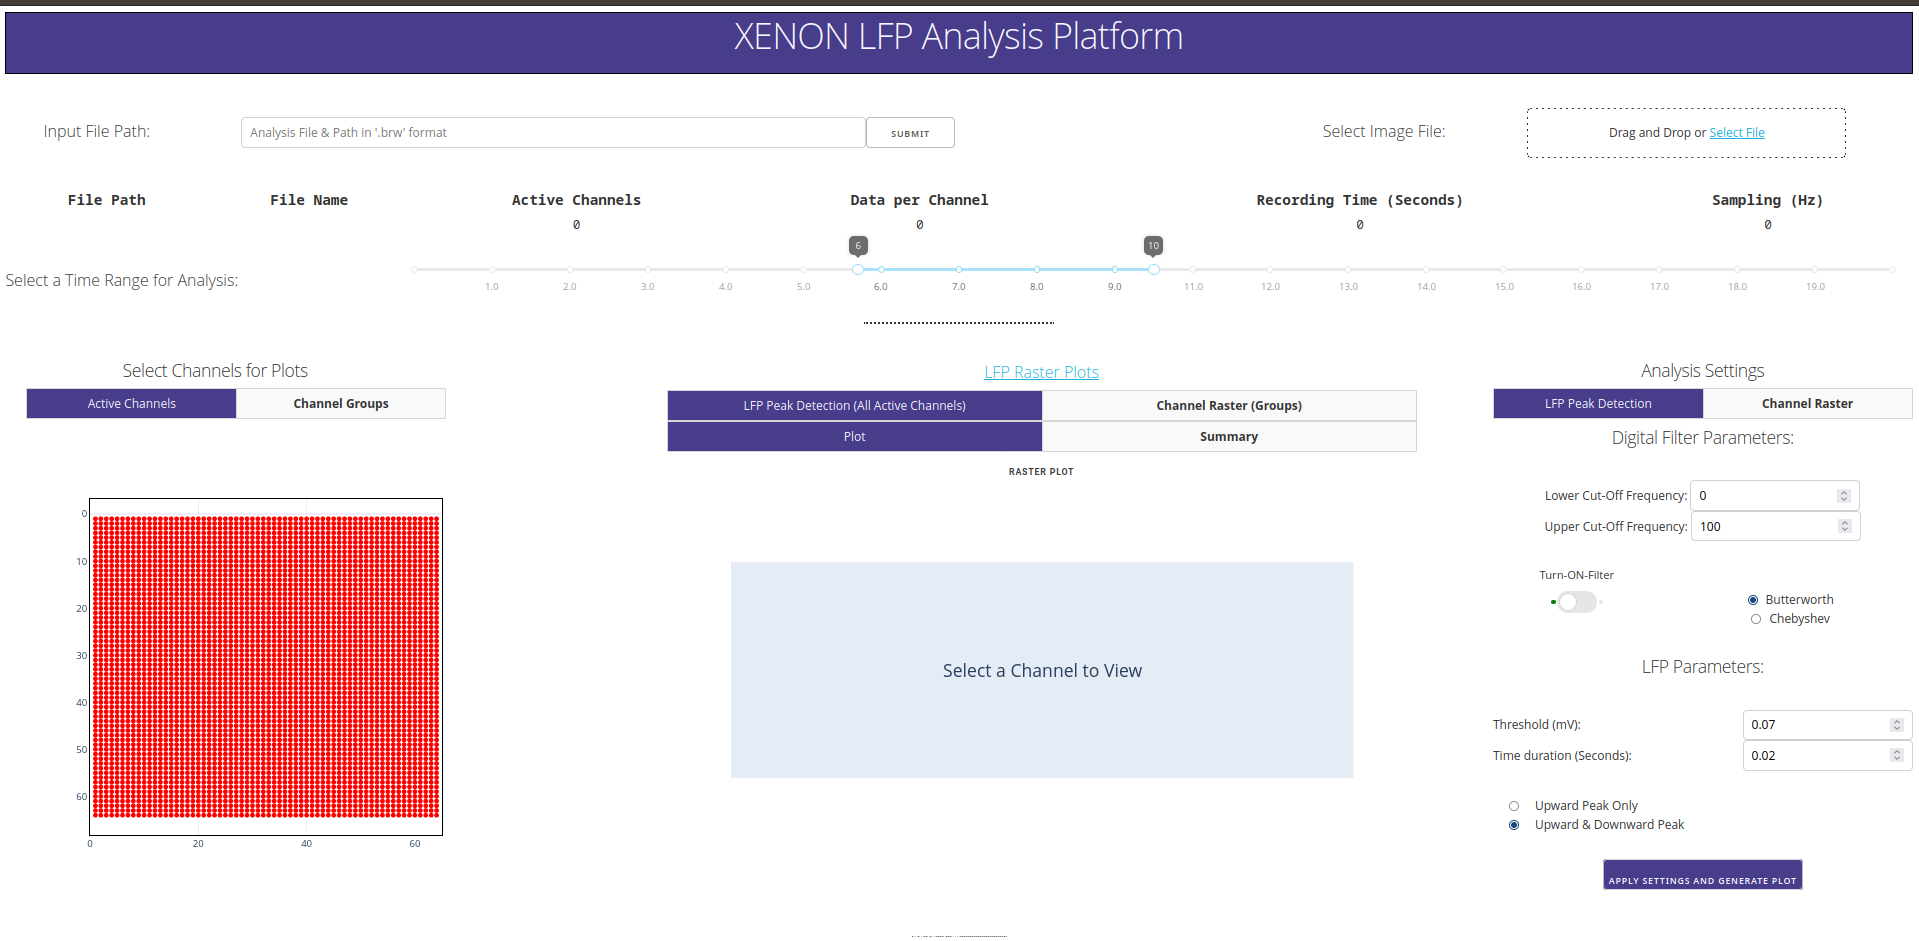
\includegraphics[keepaspectratio,width=\textwidth]{img/xenon0.png} \\
        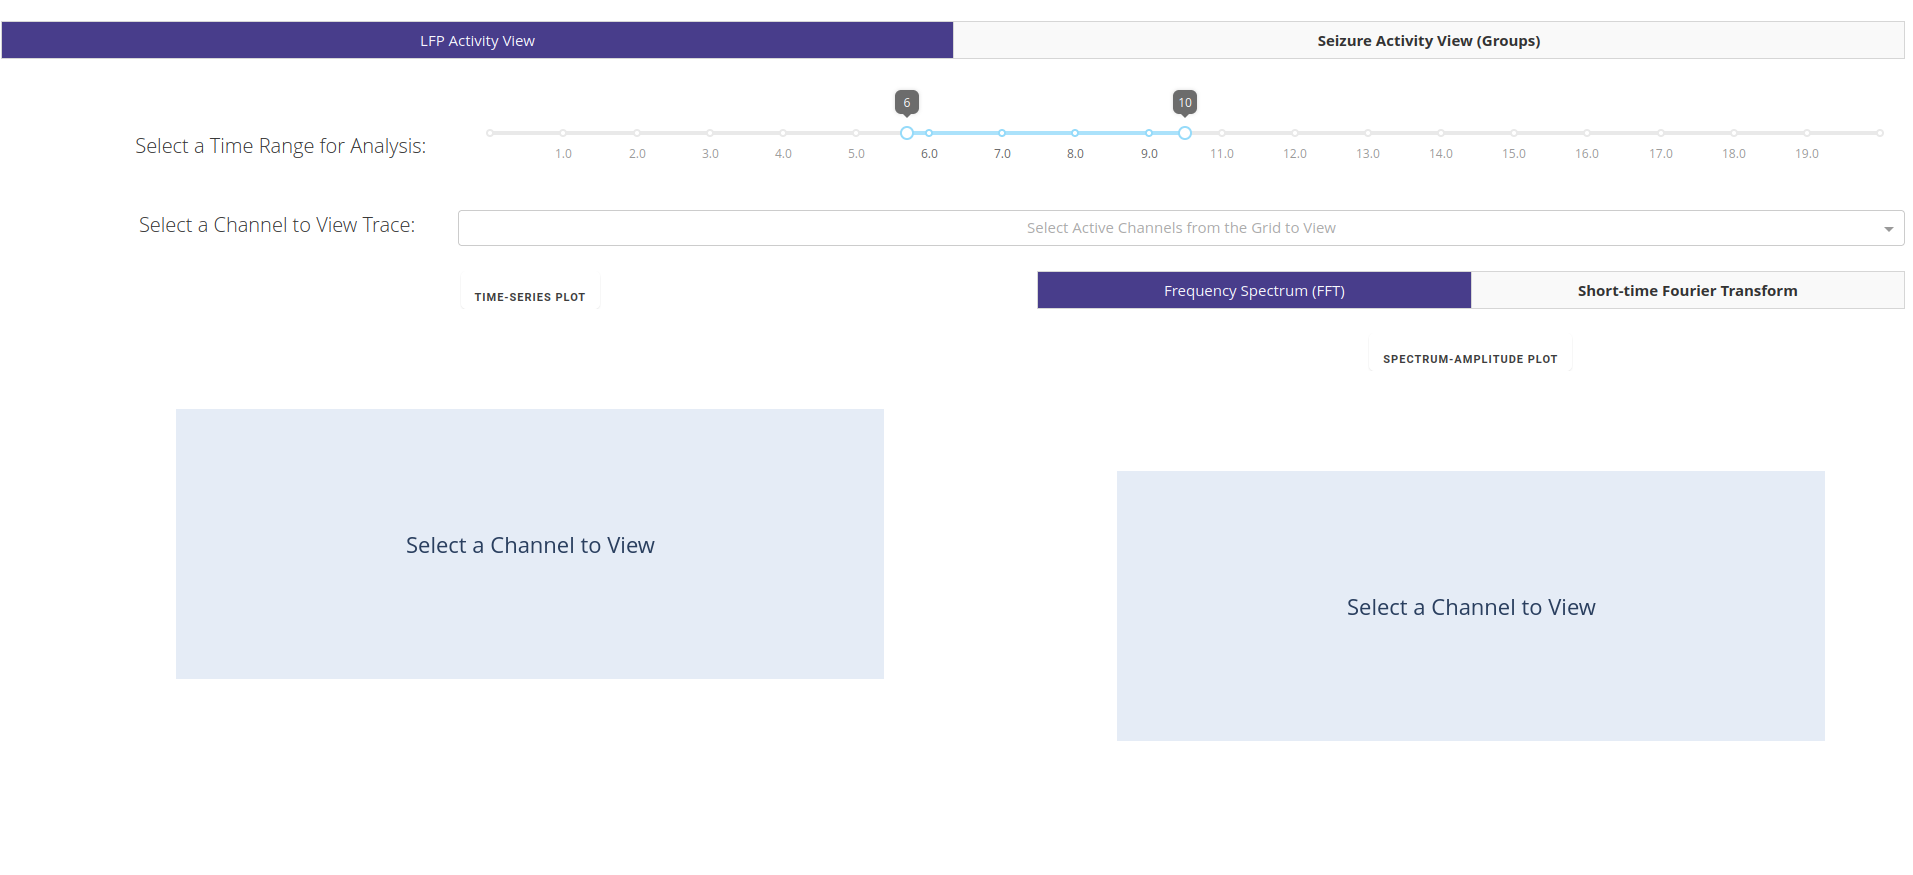
\includegraphics[keepaspectratio,width=\textwidth]{img/xenon1.png} \\
        The first function is to load a file in a certain format (.brw; a specialization of h5) as well as an microscopy image of the slice in the recording setup. 
        When the content is loaded into the RAM, the electrodes are marked on the image and it is shown to the user along with an onClick callback that lets the user select which electrodes to use or not (a click toggles if the electrode should be used).
        Additionall the user can group sets of electrodes and compare their activity by color-coding and/or groupwise aggregation of the subsequent plots.
        The time range for which data shall be considered can be set by a double slider setting start and end point in time.
        As soon as data is loaded all electrodes are selected by default, spikes are detected using the \texttt{scipy.signal.detect\_peaks} method which requires at least 2 parameters: 
        The threshold in mV defining when a part of the signal is to be considered as a peak and the time duration of the peak in seconds.
        Further the user can choose if only upwards peaks (i.e. positive change in voltage with respect to the mean) or both upwards and downwards peaks shall be considered.
        The results of the peak detection procedure is then plotted in a raster plot. 
        Additionally to the plot, the peak profiles are summarized by an aggregate over all channels, as well as the mean peak rate per second, the mean amplitude of a peak and the mean peak duration.
        Finally a bandpass filter can be applied (either Butterworth or Chebyshev).
        Both of these plots and information is updated upon a change to the channel selection, a change in the peak detection parameters and in the filter properties and application. \\
        Below these elements there are two more tabs: One for viewing the LFP activity of the individual channels and one for analyzing seizure activity.
        The LFP activity viewer allows again to select the start and end times in the signal both by double sliders and by selecting regions in the plot. 
        The plots can be zoomed in and out. 
        On selection of a subwindow, a spectrogram is shown for the selected window.
        The seizure activity view 
			
			

	\subsection{Proposed Software Design}
		In our setting, data has been recorded from a MEA with 30 $\mu$m pin electrode spacing which leaves geat doubts if the peaks in the signals do actually correspond to spikes.
		Thus non-spikes based analysis meassures shall be added to the existing piece of software.
		Also the threshold parameter varies per electrode, such that peaks should be detected independent of constant thersholds.
		The exact method to solve this is not fixed a priori but power spectal distribution based methods seem to be promising. \\
		All of the subsequent steps shall be implemented by using Dash like in Xenon's platform but using the Bootstrap extensions provided free and open source by Faculty AI. 
		This enables that each step is carried out in a separate subpage. 
		As many functions as possible shall be implemented as wrappers and GUI integration of library provided functions. \\
		
		These conditions suggest the usage of the model view controller paradigm, where the model contains data and manages their manipulation, while the controller provides means to manipulate data/the model and the view provides a visualization of the model/manipulated data. This is empoyed with a pipeline: First the data is imported, then the desired channels and time window are selected, next the signal is filtered and downsampled (to speed up computaitons). Finally transformations and analysis methods are employed and their result is visualized.
		
		\paragraph{Loading \& Focussing}
            The format that the MEA system by Multichannel system uses is called Mcs and a library to work with it is provided by the vendor. 
            So the format needs to be integrated into the existing stack by Xenon. 
            The images of Xenon are prealigned, such that displaying the electrodes is static in the sense of that the electrodes are always to be drawn at the same position. 
            The problem of aligning the pictures that have been taken from the recordings in the lab can turn out to be difficult depending on the variance in image properties and electrode visibility. \\
            As already implemented in Xenon's platform, electrode channels and time region shall be selectable dynamically.
				
		\paragraph{Preprocessing}
            The filtering with a bandpass filter shall be applicable as in Xenon's platform. 
            Additionally, the data shall be downsamplable to a user defined sampling rate.
            A reasonable default would be to downsample all raw data to 1 kHz to speed up the subsequent analysis steps.
            Further, the cleaning of noise shall be implemented in a reasonable way, to remove e.g. electric hum with a frequency of 50 Hz (EU) or 60 Hz (US), but also user defined spontaneous activity on request via graphic selection.
		
		\paragraph{Transformations \& Analysis}
            The libraries Scipy, Sklearn, Elephant, NeuroDSP, FOOOF and eventually MNE shall be used to implement the various signal processing, statistics and machine learning procedures.
            Multiple of these libraries provide functions to apply fast fourier transform, hilbert transform, short time fourier transform, morlet's wavelet transform, Granger causality, derive the envelope of the signal, cross correlation between electrodes of choice, non-negative matrix factorization, independent component analysis and more if necessarry and useful.
            FOOOF provides the possibility to split the spectrum obtained by Fourier transform variations into periodic and aperiodic components which may assist greatly in the analysis of the signal both in the frequency as well as in the time domain.
            Additionally, methods to detect peaks and bursts automatically and not based on spikes shall be derived and implemented. \\
            If there is sufficient time, and in preparation for 4096 electrode CMOS MEA recordings, SpikeInterface can be integrated to make use of a wide range of spike sorting algorithms to extend the already present tools created by the original author of the Xenon LFP Analysis platfrom.
		
		\paragraph{Visualization}
            Many of the above mentioned libraries provide functions for visualizing the raw or preprocessed signal with additionally overlaid curves or quantities like the envelope or marked brusts, raster plots of multiple of these signals with overlays as mentioned before, spectrograms, periodigrams, PSTHs and a visualization of the spreading seizure like firing patterns. The latter can be done by color coding the power of each electrode per instance in time and generating a gif such that the propagation pattern of the seizure is visible.
            
\printbibliography


\end{document}
